\subsection{Dynamik}
Die Dynamik behandelt die Kräfte als Ursache von Bewegungsabläufen. Man unterscheidet dabei die Dynamik der Translation und Rotation. (Merke: \textbf{Kraft = Gegenkraft}!)

\subsubsection{Kräfte}

\begin{itemize}
	\item Die Haft und Gleitreibung ist unabhängig von der Fläche
	\item Bei der schrägen Ebene wählt man das  Koordinaten-System mit Vorteil parallel zur Gleitebene
	\item Körper von 1kg mit $1\frac{m}{s^2}$ beschleunigen = Es wirkt eine Kraft von $1N$
	\item Beschleunigungskraft in der Schiefen Ebene: $F_B = F_H - F_G$
\end{itemize}

\begin{minipage}[h!]{0.3\linewidth}
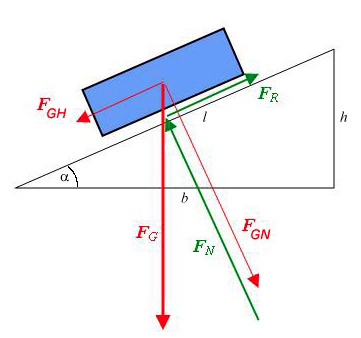
\includegraphics[width=0.9\linewidth]{images/schiefe_ebene}
\end{minipage}
\hfill
\begin{minipage}[h!]{0.2\linewidth}
	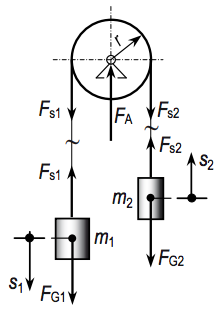
\includegraphics[width=0.9\linewidth]{images/kraefte_gleichgewicht}
\end{minipage}
\hfill
\begin{minipage}[h!]{0.4\linewidth}
\begin{align*}
m_1 \cdot a & = F_{G1} - F_{s1} \\
m_2 \cdot a & = -F_{G2} + F_{s2} \\
\Rightarrow a&=g\frac{m_1-m_2}{m_1+m_2}  \\
\Rightarrow \alpha &= \frac{a}{r} (\text{Winkelgeschwindigkeit})\\
\end{align*}
\end{minipage}

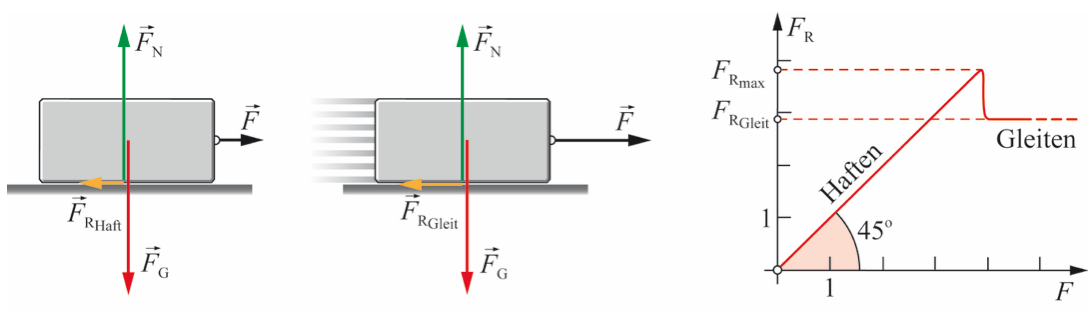
\includegraphics[width=0.9\linewidth]{images/haft_gleitkraft}


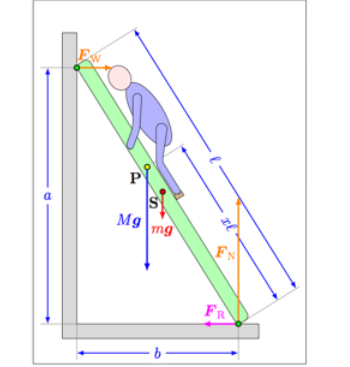
\includegraphics[width=0.3\linewidth]{images/leiter_kraefte}


\begin{tabbing}
	\begin{tabu} to \linewidth {X l X l}
		\toprule
		Kraft & $F = m \cdot a$ & 
		Kraft in Wegrichtung & $F_s = F \cos(\alpha)$ \\
		Gewichtskraft & $F_G = mg$  &
		Federkraft (Hookesches Gesetz) & $F_F = k\cdot s$ \\
		Haftreibungskraft (max) & $F_R \leq \mu_H \cdot F_N$ &
		Gleitreibungskraft & $F_R = \mu_G \cdot F_N$ \\
		Normalkraft & $F_N = mg\cdot \cos(\alpha)$ &
		Hangabtriebskraft & $F_H = F_G \cdot \sin(\alpha)$  \\
		Zentripetalkraft & $F_r = \frac{mv^2}{r} = m\omega^2r = p\omega$ & 
		Zentrifugalkraft & $F_Z = \frac{mv^2}{r} = m\omega^2r = p\omega$ \\
		Gravitationskraft & $F_G = G \cdot \frac{m_1m_2}{r^2}$
	\end{tabu}
\end{tabbing}

\begin{tabbing}
	\begin{tabu} to \linewidth {l X l}
		Variable & Bedeutung & SI-Einheit \\
		\midrule
		$F$ & Kraft & $N = \frac{kg \cdot m}{s^2}$\\ 
		$k$ & Federkonstante & $\frac{N}{m}$ \\
		$s$ & Längenänderung & $m$ \\
		$\mu_G$ & Gleitreibungskoeffizient &  \\
		$\mu_H$ & Haftreibungskoeffizient &  \\
		$G$ & Gravitationskonstante = $6.67 \cdot 10^{-11}$ & $\frac{m^3}{kg s^2}$ \\
		\bottomrule
	\end{tabu}
\end{tabbing}

\paragraph{Netwonsche Axiome}

\begin{tabbing}
	\begin{tabu} to \linewidth {l l X}
		\toprule
		I Axiom & Trägheitsprinzip & $\vec{v} = const$, wenn $ \vec{F}_{res} = \vec{0}$ \\
		II Axiom & Aktionsprinzip & $\vec{F}_{res} = m\vec{a}$\\ 
		III Axiom & Wechselwirkungsprinzip & $\vec{F}_{12} = - \vec{F}_{21}$ \\
		\bottomrule
	\end{tabu}
\end{tabbing}

\subsubsection{Arbeit}

\begin{tabbing}
	\begin{tabu} to \linewidth {l X l X}
		\toprule
		Arbeit & $W = \vec F \cdot \vec s = |\vec F| |\vec s| \cos(\alpha)\,$  &
		& \\
	\end{tabu}
\end{tabbing}

\begin{tabbing}
	\begin{tabu} to \linewidth {l X l}
		Variable & Bedeutung & SI-Einheit \\
		\midrule
		$W$ & Arbeit & $Nm = J$ \\
		$s$ & Wegstrecke & $m$ \\
		\bottomrule
	\end{tabu}
\end{tabbing}

\subsubsection{Energie}
\begin{itemize}
	\item Die Energie ist eine Zustandsgrösse eines Systems, die zunimmt, wenn von aussen Arbeit am System verrichtet wird, und die abnimmt, wenn das System nach aussen Arbeit verrichtet.
	\item Energieerhaltungssatz: Die Gesamtenergie $E_{tot}$ in einem abgeschlossenen System hat einen konstanten Wert, der von Vorgängern im Symsten nicht beeinfluss wird.
	\item Die Ausdehnung einer Feder ist proportional zur Kraft
	\item \textbf{Rollen auf der schiefen Ebene}: $E_{pot} = E_{kin} + E_{rot}$
\end{itemize}
\begin{tabbing}
	\begin{tabu} to \linewidth {l X l X}
		\toprule
		Energie & $E = P \cdot t$ & Rotationsenergie & $E_{rot} = \frac{J}{2} \cdot \omega^2 $\\
		Kinetische Energie & $E_{kin} = \frac{1}{2}mv^2$ &
		Potentielle Energie & $E_{pot} = F_G \cdot h =  mgh$ \\
		Federenergie & $E_f = \frac{F \cdot s}{2} = \frac{k \cdot s^2}{2}$ &
		Federkonstante & $k = \frac{F}{s}$ \\
	\end{tabu}
\end{tabbing}

\begin{tabbing}
	\begin{tabu} to \linewidth {l X l}
		Variable & Bedeutung & SI-Einheit \\
		\midrule
		$E$ & Energie & $J = Nm = Ws = \frac{kg \cdot m^2}{s^2}$ \\
		$k$ & Federkonstante & $\frac{N}{m}$  \\
		$s$ & Strecke welche die Feder ausgedehnt wird & $m$ \\
		$J$ & Trägheitsmoment & $J = kg \cdot m^2$ \\
		\bottomrule
	\end{tabu}
\end{tabbing}

\begin{minipage}[h!]{0.4\linewidth}
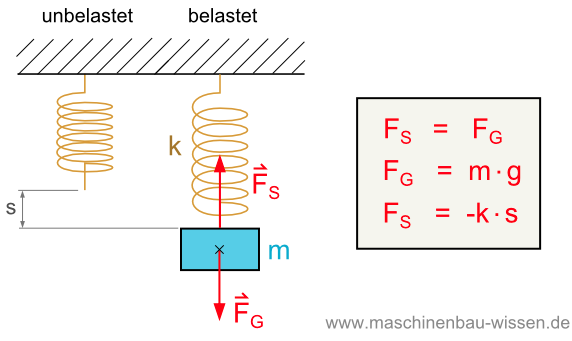
\includegraphics[width=\linewidth]{images/federenergie}
\end{minipage}
\hfill
\begin{minipage}[h!]{0.2\linewidth}
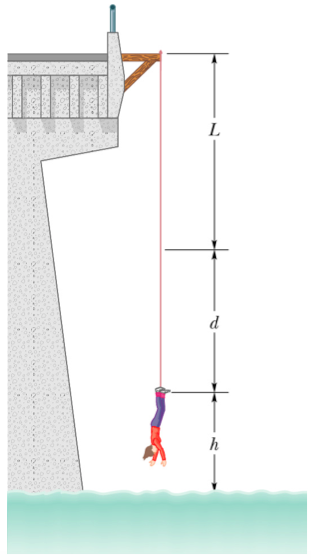
\includegraphics[width=\linewidth]{images/energie}
\end{minipage}
\hfill
\begin{minipage}[h!]{0.3\linewidth}
	\begin{align*}
	E_{pot} = E_f + E_{kin} \\
	m g (L + d) = \frac{kd^2}{2}  + \frac{m v^2}{2}  \\
	v_{Kehrpunkt} = 0 \\
	\frac{2mgL + 2mgd}{k} = d^2 \\
	d = \frac{m g}{k} \pm \frac{\sqrt{g^2 m^2 + 2 g k L m}}{k} \\
	\end{align*}
\end{minipage}

\clearpage

\subsubsection{Leistung}

\begin{tabbing}
	\begin{tabu} to \linewidth {l X l X}
		\toprule
		mittlere Leistung & $\bar{P} = \frac{W}{t}$ &
		Wirkungsgrad & $\eta = \frac{\Delta E_{ab}}{\Delta E_{zu}} = \frac{\Delta P_{ab}}{\Delta P_{zu}} < 1$ \\
		Momentanleistung & $P = F \cdot v$ & & \\
	\end{tabu}
\end{tabbing}

\begin{tabbing}
	\begin{tabu} to \linewidth {l X l}
		Variable & Bedeutung & SI-Einheit \\
		\midrule
		$P$ & Leistung & $W = \frac{J}{s} = \frac{kg \cdot m^2}{s^3}$ \\
		$E_{ab}$ & abgegebene Nutzenergie & $J$ \\
		$E_{zu}$ & aufgenommene Energie &  $J$ \\
		$W$ & verrichtete Arbeit &  $J$ \\
		$F$ & Momentankraft &  $N$ \\
		$v$ & Momentangeschwindigkeit &  $\frac{m}{s^2}$ \\
		\bottomrule
	\end{tabu}
\end{tabbing}

\paragraph{Leistung anders dargestellt}

$$P = \frac{W}{t}$$
$$W = F*s \Rightarrow P = \frac{F*s}{t}$$
$$\frac{s}{t} = v \Rightarrow P = F*v$$
$$P=\frac{\Delta E}{\Delta t}$$


\subsubsection{Impuls und Stoss}
 \textbf{Impulserhaltungssatz} In einem abgeschlossenen System bleibt der Impuls erhalten. Wenn nur Kräfte zwischen zwei Körpern wirken (Kraft = Gegenkraft) bleibt der Impuls erhalten. Die Bewegung des Schwerpunktes ändert sich nicht durch die Kollision.
 
\textbf{Elastischer Stoss}  (z.B Billiardkugel) nach dem Stoss bleibt die kinetische Energie unverändert. Der Energieerhaltungssatz für die Bewegungsenergie sowie der Impulserhaltungssatz gilt. Es geht keine Energie verloren. Der Impuls vor dem Stoss = Impuls nach dem Stoss
\begin{itemize}
	\item bewegen sich zwei Objekte aufeinander zu, ist eine Geschwindigkeit vor dem Zusammenstoss negativ.
\end{itemize}

\textbf{Unelastischer Stoss} (z.B Autounfall).
nach dem Stoss ist die kinetische Energie kleiner. (wird in Wärme und Verformungsenergie umgewandelt) (nur der Impulserhaltungssatz gilt: $p_1 + p_2 = p_1^{'} + p_2^{'}$)


\begin{tabbing}
	\begin{tabu} to \linewidth {X l X l}
		\toprule
		Impuls & $\vec{p} = m \vec{v}$  &
		Kraftstoss & $\vec{I} = \Delta \vec{p} = \vec{F} \Delta t = m \Delta \vec{v}$ \\
		Elastischer Stoss (Obj 1) & $v_1^{'} = \frac{(m_1 - m_2) \cdot v_1 + 2 m_2 v_2}{m_1+m_2}$  &
		Elastischer Stoss (Obj 2) & $v_2^{'} = \frac{(m_2 - m_1) \cdot v_2 + 2 m_1 v_1}{m_2+m_1}$ \\
		Unelastischer Stoss & $v_1^{'} = v_2^{'} = \frac{m_1v_1 + m_2v_2}{m_1 + m_2}$ & Verformungsarbeit & $W = E_1 - E_2 = \frac{m_1m_2}{2(m_1+m_2)}(v_1-v_2)^2$ \\
	\end{tabu}
\end{tabbing}

\begin{tabbing}
	\begin{tabu} to \linewidth {l X l}
		Variable & Bedeutung & SI-Einheit \\
		\midrule
		$\vec{I}$ & Kraftstoss & $Ns = \frac{kg \cdot m}{s}$ \\
		$\vec{p}$ & Impulsänderung & $Ns = \frac{kg \cdot m}{s}$ \\
		$m$ & Masse des Körpers & $kg$ \\
		$\Delta v$ & Geschwindigkeitsänderung & $\frac{m}{s}$  \\
		$F$ & beschleunigte konstante Kraft & $N$ \\
		$\Delta t$ & Dauer der Krafteinwirkung & $s$ \\
		$v^{'}$ & Geschwindigkeit des Körpers nach dem Stoss & $\frac{m}{s}$\\
		$v$ & gemeinsame Geschwindigkeit beider Körper nach dem Stoss (unelastisch) & $\frac{m}{s}$ \\
		$W$ & Verformungsarbeit & $J$\\
		$E_1$ & Summe der Bewegungsenergie beider Körper vor dem Stoss & $J$\\
		$E_2$ & Summe der Bewegungsenergie beider Körper nach dem Stoss & $J$\\
		\bottomrule
	\end{tabu}
\end{tabbing}

\paragraph{Impuls anders erklärt}

$$p = m \cdot \Delta v = m \cdot a \cdot \Delta t = F \cdot \Delta t$$

Ein Stoss überträgt Impuls, wie Arbeit Energie überträgt. Wenn man eine Kraft über eine \textit{Distanz} anwendet, macht man \textbf{Arbeit} und erhöht die \textbf{Energie}. Wenn man eine Kraft über eine \textit{Zeitdauer} anwendet, macht man einen \textbf{Stoss} und erhöht den \textbf{Impuls}.

\paragraph{Schwerpunktgeschwindigkeit}
 Die Bewegung des Schwerpunktes ändert sich nicht durch die Kollision 
 $$  u = \frac{\sum p}{ \sum m} $$

Vor dem Stoss
$$ v_{1} = u + (v_{1} -u) = u + v_{1}^{rel} $$
$$ v_{2} = u + (v_{2} -u) = u + v_{2}^{rel} $$

Elastischer Stoss
$$ v_{1} = u - (v_{1} -u) = u - v_{1}^{rel} $$
$$ v_{2} = u - (v_{2} -u) = u - v_{2}^{rel} $$
$$ E_{kin} = \frac{m_{1}+m_{2}}{2}u^2+\frac{m_{1}}{2}(v_{1}-u)^2+\frac{m_{2}}{2}(v_{2}-u)^2 $$

Inelastischer Stoss
$$ v_{1}=v_{2}=u $$
$$ E_{kin} = \frac{m_{1}+m_{2}}{2}u^2$$

\paragraph{Vollkommen inelastischer Stoss}
Die Objekte bewegen sich nachher gemeinsam weiter. Impuls ist vor und nach dem Stoss gleich

Deformationsenergie
$$ Q = E_{kin1} + E_{kin2} - (E_{kin1}^{\prime}  + E_{kin2}^{\prime})  $$

\subsubsection{Dynamik der Drehbewegung}
\begin{itemize}
	\item Zentripetalkraft (Ursache für Zentralbewegung) und Zentrifugalkraft (Fliehkraft) sind gleich gross, aber entgegengerichtet.
	\item Trägheitsmoment: Bei einem drehbaren Körper ist das Verhältnis von wirkendem Drehmoment zur erzielten Winkelbeschleunigung eine konstante Grösse, dem Trägheitsmoment.
\end{itemize}
\begin{tabbing}
	\begin{tabu} to \linewidth {X l X l}
		\toprule
		Trägheitsmoment & $J = r^2\Delta m$ &
		Trägheitsmoment & $J = \sum_{i=1}^{n}r_i^2 \Delta m_i$ \\
		Zentripetalkraft & $F_r = F_z = \frac{mv^2}{r} = m\omega^2r = p\omega$ & 
		Zentripetalbeschl & $a_r = a_z = r \omega^2 = \frac{v^2}{r}$ \\
		Rotationsleistung & $P = M \omega$ &
		Rotationenergie & $E_{rot} = \frac{J\omega^2}{2}$\\
		Drehmoment & $M = J\alpha$ &
		Rotationsarbeit & $W = M\varphi$ \\
		Drehimpuls & $L = J \omega = M \cdot t = r\cdot p$ & 
		Drehimpuls einer Punktmasse & $\Delta M = \frac{\Delta L}{\Delta t}$ \\
	\end{tabu}
\end{tabbing}

\begin{tabbing}
	\begin{tabu} to \linewidth {l X l}
		Variable & Bedeutung & SI-Einheit \\
		\midrule
		$J$ & Trägheitsmoment & $J = kg \cdot m^2$ \\ 
		$m$ & Masse eines dünnen Kreisringes (Umfang) & $kg$ \\ 
		$r$ & einheitlicher Abstand aller Massenelemente von der Drehachse & $m$ \\ 
		$m_i$ & Massenelement & $kg$\\ 
		$P$ & Leistung & $W$ \\ 
		$p$ & Impuls des Körpers & $N \cdot s$ \\
		$M$ & Drehmoment, das die Drehung verursacht & $N \cdot m$ \\ 
		$\omega$ & Winkelgeschwindigkeit des Körpers & $\frac{rad}{s} = \frac{1}{s}$ \\ 
		$L$ & Drehimpuls des rotierenden Körpers & $\frac{kg \cdot m^2}{s} = N \cdot m \cdot s$  \\ 
		$\alpha$ & Winkelbeschleunigung & $\frac{rad}{s^2} = \frac{1}{s^2}$ \\
		\bottomrule
	\end{tabu}
\end{tabbing}



\begin{minipage}[h!]{0.5\linewidth}
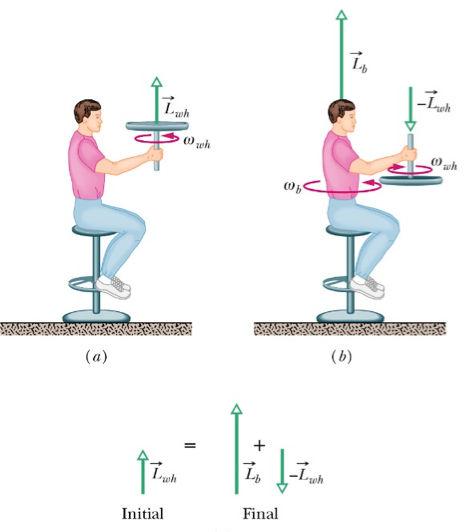
\includegraphics[width=0.8\linewidth]{images/drehimpuls}
\end{minipage}
\hfill
\begin{minipage}[h!]{0.5\linewidth}
	\begin{align*}
		L_b &= J_b \omega_b \\
		L_{wh} &= J_{wh} \omega_{wh} \\
		L_{wh} &= L_b - L_{wh} \\
		J_{wh} \omega_{wh} &= J_b \omega_b - J_{wg} \omega_{wg} \\
		\omega_b &= \frac{2J_{wh}}{J_b} \omega_{wg} \\
	\end{align*}
\end{minipage}